\documentclass{beamer}

\title{PageRank}
\author{Ben Burns, Dan Magazu, Lucas Chagas, \\Thomas Webster, Trung Do}
\date{Fall 2021}

\usepackage{outlines}
\usepackage{graphicx}
\usepackage{amsmath}
\usepackage{color, xcolor, mdframed}

\graphicspath{{./images}}

\addtobeamertemplate{navigation symbols}{}{%
    \usebeamerfont{footline}%
    \usebeamercolor[fg]{footline}%
    \hspace{1em}%
    \insertframenumber/\inserttotalframenumber
}

%\AtBeginSection[ ]
%{
%\begin{frame}{Outline}
%    \tableofcontents[currentsection]
%\end{frame}
%}

\begin{document}

\frame{\titlepage}

\begin{frame}
\frametitle{Table of Contents}
\tableofcontents
\end{frame}

\section{Motivation}
\begin{frame}[t]
\frametitle{Motivation}
\begin{itemize}
    \setlength\itemsep{0.5em}
    \item Problem: the internet has a \emph{lot} of web pages
    \item A lot of the information out there either isn't relevant to us, or is inaccurate
    \item Motivation: we want a program that, when provided a phrase, returns webpages with information relevant to the input
    \item Intuitive solution: return back websites that either contain that phrase, or contain similar phrases
    \item This helps us find more \emph{relevant} pages, but we can't know if we're getting the best information (much less \emph{accurate} information) without manually going through each result
    \item We desire a stronger solution
\end{itemize}
\end{frame}

\section{Background}
\begin{frame}[t]
\frametitle{PageRank}
\begin{outline}
    \1 Invented by Sergey Brin and Larry Page (1998)\footnotemark 
        \2 Publication marks them becoming co-founders of Google  
    \1 Idea: we want some way to numerically score each webpage based on how "important" it is
    \1 Algorithm numerically scores each page $p$ based on 
        \2 How many other pages link to $p$ (or "cite" it)
        \2 The "importance" of each of $p$'s citations 
    \1 We then numerically order pages to rank them
    \1 PageRank: the procedure for scoring each website
    \1 Google: the database that indexes the PageRank of each website for search
\end{outline}
\footnotetext[1]{Many use the year of the original manuscript, 1996}
\end{frame}

\begin{frame}[t]
\frametitle{Underlying Assumptions}    
\begin{outline}
    \1 Running our basic search engine gives us a collection of pages with information relevant to our query
    \1 Assumption: More "important" and useful websites will be the ones with proportionally more inbound links
    \1 Pages with very reliable, primary information are likely to be cited by lots of website authors, and therefore will have lots of "flow" into them
    \1 Assumption: websites with no outgoing links are treated as linking to every other website
    \1 Else, these pages would just take in flow without ever redistrubting, and eventually all users get stuck on these pages
\end{outline}
\end{frame}

\begin{frame}[t]
\frametitle{Finding Less Important Information}
\begin{outline}
    \1 A worry you may have is that we'll only find pages with lots of inbound links
    \1 You can still find niche information by making your query more specific so that it won't match more general pages
    \1 Searching "PageRank" will likely get you Wikipedia, but "Anatomy of PageRank architecture" gives you the original research literature. 
    \1 Your returned urls are still proportionally important results, your query just filtered out the numerically more "important", yet less relevant pages.
\end{outline}
\end{frame}

\section{Formalizing PageRank}
\begin{frame}[t]
\frametitle{Formalizing the PageRank problem}
\begin{outline}
    \1 We're going to construct a directed graph $G = (V, E)$
    \1 For each website we consider, we construct a node $v_i \in V$
    \1 For two distinct nodes $v_i,\ v_j \in V$, the \emph{directed} edge $v_iv_j \in E$ iff there is a link on website $i$ that goes to website $j$.
    \1 If $v_i$ and $v_j$ are not distinct (a website is linking to itself), we ignore the link and do not construct a loop edge.
        \2 $G$ is not a psuedograph
    \1 Multiple hyperlinks on page $i$ to page $j$ are all represented by the single, directed edge 
        \2 $G$ is not a multigraph.
\end{outline}
\end{frame}

\begin{frame}
\frametitle{Visual Representation}
\begin{center}
    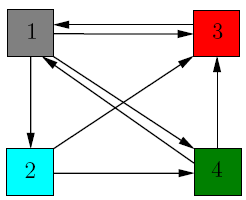
\includegraphics[width=0.6\textwidth]{unweighted.png}
\end{center}
\begin{outline}
    \1 We have a set of 4 websites
    \1 Each edge represents a hyperlink from the origin node to the destination node 
\end{outline}
\end{frame}

%\begin{frame}{Adjacency Matrix}
%\begin{columns}
%    \begin{column}{0.5\textwidth}
%        \centering
%        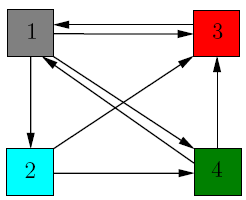
\includegraphics[width=\textwidth]{unweighted.png}
%    \end{column}
%    \begin{column}{0.5\textwidth}
%        \centering
%        {\Large$A = \begin{pmatrix}
%            0 & 1 & 1 & 1\\
%            0 & 0 & 1 & 1\\
%            1 & 0 & 0 & 0\\
%            1 & 0 & 1 & 0\\
%        \end{pmatrix}$}
%    \end{column}
%\end{columns}
%\begin{outline}
%    \1 No self loops means the main diagonal is all zeros
%\end{outline}
%\end{frame}

\begin{frame}[t]
\frametitle{Applying PageRank Values}
\begin{outline}
    \1 At first, we assign each vertex $v\in V$ with a weight of $\dfrac{1}{|V|}$. 
    \1 All vertices have equal weight, and our weights sum up to 1. The weight of a particular vertex $v_i$ is denoted $PR(v_i)$.
    \1 Consider the set $O_i$ of vertices that $v_i$ has an edge to:
        \2 $O_i = \{v_j | v_iv_j \in E\}$ ($O$ for outbound)
    \1 A user on page 1 can choose to click a link to traverse to either 2, 3, or 4. In other words, $O_1 = \{2, 3, 4\}$.
\end{outline}
\begin{center}
    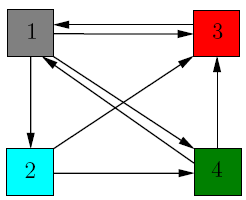
\includegraphics[width=0.4\textwidth]{unweighted.png}
\end{center}
\end{frame}

\begin{frame}[t]
\frametitle{Traversing from Page to Page}
\begin{itemize}
    \setlength\itemsep{1em}
    \item Assumption: A user on page $i$ user is equally likely to choose to visit each vertex in $O_i$ (our set of vertices that $v_i$ cites)
    \item In our example from before, the probabilty that our user on page 1 visits page 2 is $P(v_2) = \dfrac{1}{|O_1|} = \dfrac{1}{3}$
    \item So a third of page 1's visitors will "flow" to page 2, a third to page 3, and a third to page 4
    \item From $v_i$, $P(v_j) = \dfrac{1}{|O_i|}$ if $v_j \in O_i$, and 0 else.
\end{itemize}
\end{frame}

\begin{frame}[t]
\frametitle{Iteration Model}
\begin{outline}
    \1 All at once, all users will click one of the links on their current page
    \1 At "click 0", the PageRank value of all vertices $PR(v, 0) = \dfrac{1}{|V|}$
    \1 On click 1, each page will equally split its PageRank value among the pages it cites
    \1 Page 1 starts with $PR(v_1, 0) = \dfrac{1}{4}$, and contributes $\dfrac{1}{12}$ to each of 2, 3, and 4 on click 1
    \1 Conversely, page 1 will receive nothing from page 2, all of $PR(v_3, 0)$, and half of $PR(v_4, 0)$. So after click 1, 
    \begin{align*}
        PR(v_1, 1) &= 0\cdot PR(v_2, 0) + PR(v_3, 0) + \dfrac{1}{2}PR(v_4, 0) \\
        &= \dfrac{1}{4} + \dfrac{1}{8} = \dfrac{3}{8}\\
    \end{align*}
\end{outline}
\end{frame}

%\begin{frame}{Example iterations}
%\bgroup
%\def\arraystretch{2.5}
%\begin{tabular}{|c|c|c|c|c|c|c|c|c|}
%    \hline
%    $PR$ & 0 & 1 & 2 & 3 & 4 & 5 & 6 & 7\\
%    \hline
%    $v_1$ & $\dfrac{1}{4}$ & $\dfrac{3}{8}$ & $\dfrac{7}{16}$ & 0.3542 & 0.3958 & 0.3906& 0.3819 & 0.3898\\
%    $v_2$ & $\dfrac{1}{4}$ & $\dfrac{1}{12}$ & $\dfrac{1}{8}$ & 0.1458 & 0.1181 & 0.1319& 0.1302 & 0.1273\\
%    $v_3$ & $\dfrac{1}{4}$ & $\dfrac{1}{3}$ & $\dfrac{13}{48}$ & 0.2917 & 0.2951 & 0.2865& 0.2917 & 0.2905\\
%    $v_4$ & $\dfrac{1}{4}$ & $\dfrac{5}{24}$ & $\dfrac{1}{6}$ & 0.2083 & 0.1910 & 0.1910 & 0.1962 & 0.1924\\
%    \hline
%\end{tabular}
%\egroup
%\end{frame}

\begin{frame}[t]{What else do we need?}
    \begin{outline}
        \1 We want a function $f(v_i, v_j)$ defined as:
        \begin{mdframed}[backgroundcolor=blue!20]
            \begin{center}
                $f(v_i, v_j) := \dfrac{\text{\# of links from page }i\text{ to page }j}{\text{total \# of links out of page }j}$        
            \end{center}    
        \end{mdframed}
        \1 In our simplified case, this will be $\dfrac{1}{|O_j|}$ if $j$ links to $i$, and 0 else
        \1 Additionally, at some point, our user who is randomly clicking links will eventually stop clicking links
        \1 At each iteration we consider a constant probability\\ $d :=$ the probability that our user stops traversing the graph
            \2 Various studies have settled on $d\approx 0.85$
    \end{outline}
\end{frame}

\begin{frame}[t]
\frametitle{General PageRank equation}
\begin{outline}
    \1 For an arbitrary graph, we obtain the PageRank value of vertex $v_i$ at iteration $t + 1$ from the following: 
    \begin{mdframed}[backgroundcolor=blue!20]
        \begin{center}
            \begin{math}
                PR(v_i, t+1) = \dfrac{1-d}{|V|} + d\sum\limits_{v_j \in I_i} f(v_i, v_j) PR(v_j, t)
            \end{math}
        \end{center}
    \end{mdframed}
    \vspace{1em}

    \begin{tabular}{cc}
        $O_i$ is set of vertices with & $I_i$ is the set of vertices with \\
        edges outbound from $v_i$ & edges inbound to $v_i$\\
    \end{tabular}

    \vspace{1em}

    \begin{center}
        $f(v_i, v_j)=\begin{cases} 
            \dfrac{1}{|O_j|} & i \in O_j\\
            0 & \text{else} 
         \end{cases}$\\
    \end{center}
\end{outline}
\end{frame}

%\begin{frame}{Iterations w/ Damping}
%\bgroup
%\def\arraystretch{2.5}
%\begin{tabular}{|c|c|c|c|c|c|c|c|c|}
%    \hline
%    $PR$ & 0 & 1 & 2 & 3 & 4 & 5 & 6 \\%& 7\\
%    \hline
%    $v_1$ & $\dfrac{1}{4}$ & 0.3562 & 0.4014 & 0.3502 & 0.3720 & 0.3697 & 0.3664\\% & 0.3689\\
%    $v_2$ & $\dfrac{1}{4}$ & 0.1083 & 0.1384 & 0.1512 & 0.1367 & 0.1429 & 0.1422\\% & 0.1413\\
%    $v_3$ & $\dfrac{1}{4}$ & 0.3208 & 0.2757 & 0.2885 & 0.2903 & 0.2864 & 0.2884\\% & 0.2880\\
%    $v_4$ & $\dfrac{1}{4}$ & 0.2146 & 0.1845 & 0.2101 & 0.2010 & 0.2010 & 0.2030\\% & 0.2018\\
%    \hline
%\end{tabular}
%\egroup
%\begin{itemize}
%    \item Looks okay, but the values don't quite converge
%\end{itemize}
%\end{frame}

\section{Solving PageRank as a Matrix}
\begin{frame}[t]{Matrix Construction}
\begin{outline}
    \1 The idea behind PageRank is construct and solve a matrix
    \1 Each row $i$ represents the PageRank equation for $PR(v_i, t)$ 
    \1 Each column $j$ represents the PageRank value contributed by $j$ to each vertex $v_i$
    \1 The solved for $t+1$ iteration PageRank values will therefore be a vector:
    \begin{center}
        \begin{math}
            \begin{bmatrix}
                PR(v_1, t+1)\\
                PR(v_2, t+1)\\
                \vdots\\
                PR(v_n, t+1)\\
            \end{bmatrix}
        \end{math}
    \end{center}
\end{outline}
\end{frame}

\begin{frame}[t]{Boiling it Down to an Eigenvalue}
\begin{outline}
    \1 For our iteration process, we want to be able to input a vector of PageRank values at iteration $t$ vector $\mathbf{R}(t)$, and get back a vector of PageRank values at iteration $t+1$ ($\mathbf{R}(t+1)$)
    \1 In other words, we can determine PageRank values as 
    \begin{center}
        \begin{math}
            \begin{bmatrix}
                PR(v_1, t+1)\\
                PR(v_2, t+1)\\
                \vdots\\
                PR(v_n, t+1)\\
            \end{bmatrix} = A\cdot \begin{bmatrix}
                PR(v_1, t)\\
                PR(v_2, t)\\
                \vdots\\
                PR(v_n, t)\\
            \end{bmatrix}
        \end{math}
    \end{center}
    for an $n\times n$ matrix $A$ 
    \1 For our values to converge, our input vector will approximately equal our output vector 
    \1 In other words, we're searching for an eigenvector
\end{outline}
\end{frame}

\begin{frame}[t]{Defining Our Matrix $A$}
    \begin{outline}
        \1 Observe our general PageRank equation
        \begin{mdframed}[backgroundcolor=blue!20]
            \begin{center}
                \begin{math}
                    PR(v_i, t+1) = \dfrac{1-d}{|V|} + d\sum\limits_{v_j \in I_i} f(v_i, v_j) PR(v_j, t)
                \end{math}
            \end{center}
        \end{mdframed}
        \1 We define the matrix $A$ to the $n\times n$ matrix where $A_{ij}:= f(v_i, v_j)$
        \1 We then multiply this matrix by our $t$ iteration PageRank vector
        \1 Finally, we add the result by a $n$ length vector of $\dfrac{1-d}{|V|}$ terms
        \begin{center}
            \begin{math}
                \mathbf{R}(t+1) = \begin{bmatrix}
                    (1-d)/|V|\\
                    (1-d)/|V|\\
                    \vdots\\
                    (1-d)/|V|\\
                \end{bmatrix} + \begin{bmatrix}
                    f(v_1, v_1) & \ldots &f(v_1, v_n)\\
                    f(v_2, v_1) & \ldots &f(v_2, v_n)\\
                    \vdots & \ddots & \vdots \\
                    f(v_n, v_1) & \ldots &f(v_n, v_n)\\
                \end{bmatrix}\cdot \mathbf{R}(t)
            \end{math}
        \end{center}
    \end{outline}
\end{frame}

\begin{frame}[t]{Determining Existance of $PR$ Eigenvector}
    \begin{outline}
        \1 Each column $j$ of our matrix is the series of terms $f(v_1, v_j)$ through $f(v_n, v_j)$
        \1 Recall that $f$ is defined as 
        \begin{center}
            $f(v_i, v_j)=\begin{cases} 
                \dfrac{1}{|O_j|} & i \in O_j\\
                0 & \text{else} 
             \end{cases}$\\
        \end{center}
        \1 All entries are non-negative
        \2 $|O_j|$ entries will hold a value of $\dfrac{1}{|O_j|}$
        \2 All other values will be zero
        \1 Further, the sum of the entries in any column $j$ is 
        \begin{center}
            $\sum\limits_{v_i \in V} f(v_i, v_j) = |O_j|\dfrac{1}{|O_j|} = 1$            
        \end{center}
        and $A$ is column stochasic matrix
    \end{outline}
\end{frame}

\begin{frame}[t]{Perron-Frobenius Theorem}
    \begin{outline}
        \begin{mdframed}[backgroundcolor=blue!20]
            \textbf{Perron-Frobenius Theorem}: \\If $A$ is a positive, column stochastic matrix, then\\
            1. 1 is an eigenvalue of multiplicity one.\\
            2. 1 is the largest eigenvalue: all the other eigenvalues have absolute value smaller than 1.\\
            3. the eigenvectors corresponding to the eigenvalue 1 have either only positive entries or only negative entries. In particular, for the eigenvalue 1 there exists a unique eigenvector with the sum of its entries equal to 1.\\
        \end{mdframed}
    Using this theorem, $Av = v$ will always have the (largest) eigenvalue equal 1.
    \end{outline}
\end{frame}

\section{Applications}
\begin{frame}[t]
    \frametitle{Applications}
    \begin{outline}
        \1 PageRank is perhaps the most famous search ranking algorithm. Googles high-quality search engine results are directly correlated to PageRank
        \1 There are a remarkable wide variety of applications of the PageRank algorithm that apply to non-search engine contexts.
        \1 Its simplicity and elegance allow PageRank to be a more general and powerful tool.
        \1 Let's look at the applications of PageRank and its connection to Twitter.

    \end{outline}
\end{frame}

\begin{frame}[t]
    \frametitle{Twitter}
    \begin{outline}
        \1 In 2010, Twitter was lagging behind and was lacking a user recommendation service. 
        \1 This was perceived both externally and internally as a critical gap in Twitter’s product offerings, so quickly launching a high-quality product was a top priority.
        \1 Twitter is unique because of the asymmetric nature of the following relationship—a user can receive messages from another without reciprocation. 
        \1 This differs substantially from other social networks such as Facebook or LinkedIn, where social ties can only be established with the consent of both participating members.
    \end{outline}
\end{frame}

\begin{frame}[t]
    \frametitle{Introducing PageRank}
    \begin{outline}
        \1 This works well with PageRank because we can determine outbound and inbound links.
        \1 A user $u$ is likely to follow those who are followed by users that are similar to $u$. 
        \1 These users are in turn similar to $u$ if they follow the same (or similar) users.
        \1 Therefore using Page Rank, Twitter is able to offer unique recommendations for users. 
        \1 By analyzing who the user follows and who those users follow, the PageRank algorithm will allow Twitter to make specific recommendations for each user. 
        \1 Essentially, the more outbound links that an account receives correlate to a higher PageRank score.        
    \end{outline}
\end{frame}
%\begin{frame}
%\frametitle{Visual Representation}
%\begin{center}
%    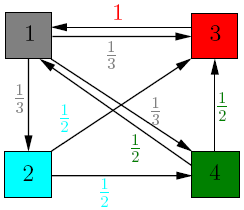
\includegraphics[width=0.6\textwidth]{weighted.png}
%\end{center}
%\begin{outline}
%    \1 In this case, all nodes have a PageRank value of 1.
%\end{outline}
%\end{frame}


\end{document}